\chapter{Design und Konzeption}\label{design-konzeption}
Nach der Analyse der Aufgabenstellung und der Erarbeitung des Knowhows im Bereich von Scala und Lift ging es an Design und Konzeption. In dieser Phase entstanden auf der Basis der Use Cases das Konzept der Benutzerrollen, der Navigation und das Design der Prozesse. Als Basis f\"ur die Implementation diente das am Ende beschriebene Entity Relationship Model.\section{Use Cases Beschreibung}\label{konzept:usecase}
 \begin{figure}[H]
  	\centering
    	\fbox{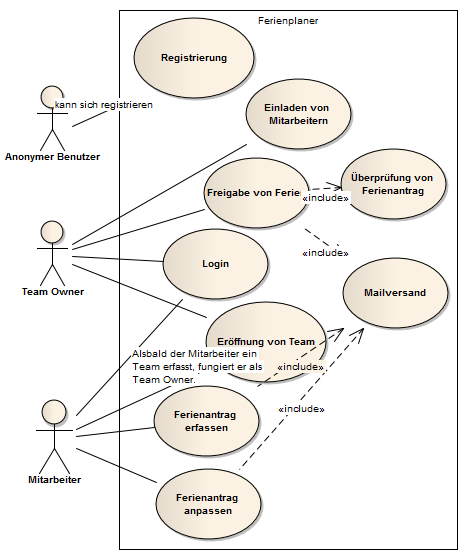
\includegraphics[width=13cm]{images/usecases}}
 	\caption{Use Case Diagramm}
\end{figure}
\subsection{Aktoren}
\subsubsection{Mitarbeiter} sind registrierte Benutzer und k\"onnen von Team Ownern zu den entsprechenden Teams hinzugef\"ugt werden. 
\subsubsection{Owner - Team Owner} sind grunds\"atzlich auch Mitarbeiter, die allerdings ein eigenes Team administrieren und f\"ur dieses (es k\"onnen auch mehrere sein) deshalb zus\"atzliche Kompetenzen besitzen.

\subsection{Beschreibung der Use Cases}
\subsubsection{Projekt er\"offnen}
Nach dem Login erfasst der Administrator (Project Manager, Teamleiter, usw.) f\"ur sein Team ein Projekt. Grunds\"atzlich kann ein Projekt mehreren Administratoren besitzen. Ich werden diesen Fall aber nicht ber\"ucksichtigen und anstelle nur einem Administrator zuweisen.
\subsubsection{Mitarbeiter in Projekt erfassen}
Projekte alleine dienen der Gruppierung der Mitarbeiter, anhand dieser werden die Berechtigungen f\"ur die Administratoren gegeben. Um Mitarbeiter ins eigene Projekt zu nehmen, sucht der Administrator nach einem bestehenden User. Eine zus\"atzliche M\"oglichkeit w\"are die direkte Erfassung der Mitarbeiter und entspechende Validierung durch den Betroffenen.
\subsubsection{Ferienw\"unsche bearbeiten}
Die vom Mitarbeiter erfassten Ferien k\"onnen durch den Administrator bez\"uglich Status und Termin ver\"andert werden. Die Bewilligung von Ferien wird mittels des Status confirmed / best\"atigt erteilt. Ansonsten gibt es folgende M\"oglichkeiten:
\begin{itemize}
\item erw\"unscht - requested
\item abgelehnt - rejected
\item best\"atigt - confirmed
\end{itemize}

\subsubsection{Ferienwunsch erfassen}
Der Mitarbeiter kann seine Ferienw\"unsche pro Projekt erfassen. Diese befinden sich zu Beginn im Status ''requested'' und k\"onnen vom Administrator in die Status ''rejected'' und ''confirmed'' ge\"andert werden. Falls der Mitarbeiter sich in mehreren Projekten befindet muss er aufgrund der Zust\"andigkeit f\"ur beide einen Antrag stellen.

\subsubsection{Ferienwunsch bearbeiten}
Sollte ein Ferienwunsch abgelehnt werden, kann er erneut bearbeitet werden. Jede \"Anderung wird allen beteiligten per Mail mitgeteilt.

\section{Rollen-Konzept}\label{konzept:rollen}
Im Grunde handelt es sich bei dem Ferienplaner um einen Prototypen ohne eigentliche Gesch\"aftsidee. Es war einfach eine Gute Aufgabenstellung um sich das Lift Framework und Scala anzusehen. Aus diesem Grund sehe ich als Anfang nur 2 Rollen vor. Zum einen ist es der Anonyme Benutzer, der zwar die Webseite Besuchen kann, sich f\"ur die weiteren Schritte allerdings registrieren muss, zum anderen ist es der Registrierte Benutzer, der nicht nur Ferien erfassen, sondern auch eigene Teams mit eigenen Mitarbeitern bilden kann.
\subsection{Anonymous}
Folgende Funktionalit\"aten stehen dem Anonymous zur Verf\"ugung:
\begin{itemize}
\item Ansicht von \"offentlichen Seiten
\item Registrierung
\end{itemize}

\subsection{Registrierte Benutzer}
Nebst den Funktionen des Anonymous stehen dem Registrierten Benutzer folgende Dinge zur Auswahl:
\begin{itemize}
\item Login
\item Administration von Teams und Zuweisung von Mitarbeitern
\item Einladen von Mitarbeitern
\item Erfassen von Ferien f\"ur Teams welchen der Registrierte Benutzer angeh\"ort.
\end{itemize}

\subsection{Optional Aufteilung der Registrierten Benutzer}
Es best\"unde in einem weiteren Schritt die M\"oglichkeit, die Rolle des Registrierten Benutzers in Mitarbeiter und Team Owner aufzuteilen. In diesem Falle h\"atte man die M\"oglichkeit, eine Kostenpflicht zu implementieren. Als Beispiel w\"urden die Rollen folgendermassen aussehen:
\subsubsection{Mitarbeiter}
Folgende Funktionalit\"aten stehen dem Mitarbeiter zur Verf\"ugung:
\begin{itemize}
\item Erfassen von Ferien f\"ur Teams welchen der Registrierte Benutzer angeh\"ort.
\end{itemize}

\subsubsection{Team Owner}
Zus\"atzlich zu den Funktionen des Mitarbeiters kann der Team Owner folgendes tun:
\begin{itemize}
\item Administration von Teams und Zuweisung von Mitarbeitern
\item Einladen von Mitarbeitern
\end{itemize}

\section{Prozesse}\label{konzept:prozesse}
\subsection{Person registrieren}
 \begin{figure}[H]
  	\centering
    	\fbox{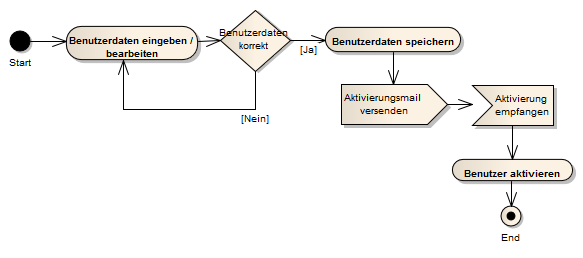
\includegraphics[width=15cm]{images/process_registration}}
 	\caption{Prozess Member Administration Webpage}
\end{figure}

\subsection{Ferien beantragen, planen}\label{prozess:ferien}
 \begin{figure}[H]
  	\centering
    	\fbox{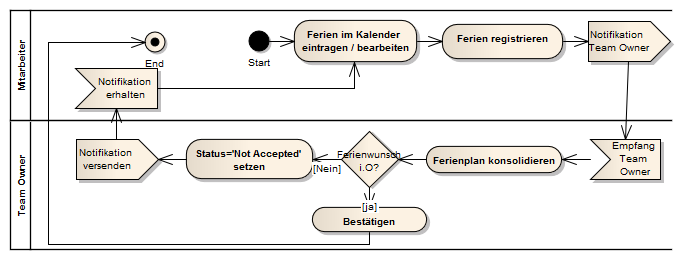
\includegraphics[width=15cm]{images/process_vacation}}
 	\caption{Prozess Ferien beantragen, planen}
\end{figure}


\subsection{Team administrieren}\label{prozess:team}
 \begin{figure}[H]
  	\centering
    	\fbox{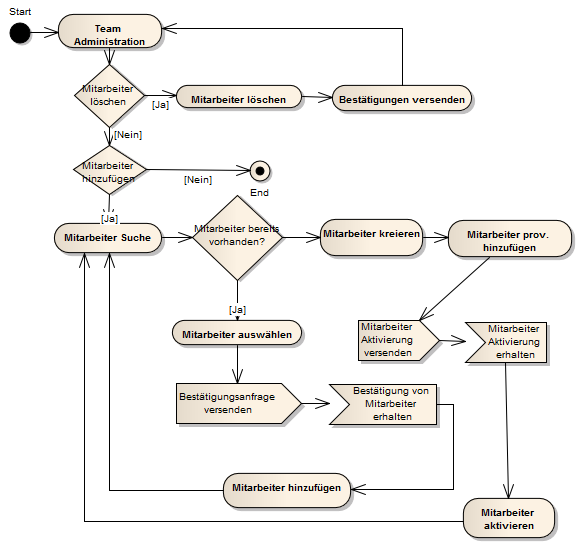
\includegraphics[width=15cm]{images/process_team_administration}}
 	\caption{Prozess Member Administration Webpage}
\end{figure}

\section{Navigations-Konzept}\label{konzept:navigation}
 \begin{figure}[H]
  	\centering
    	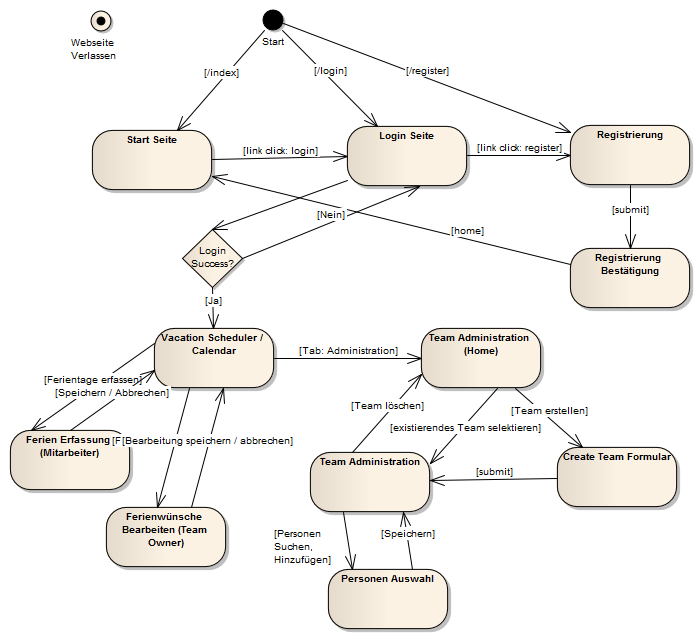
\includegraphics[width=13cm]{images/navigation_process}
 	\caption{Navigation Webpage}
\end{figure}

\section{Datenbank-Schema}\label{design:erm}

\subsection{Entity Relationship Model}
\begin{landscape}
 \begin{figure}
  	\centering
    	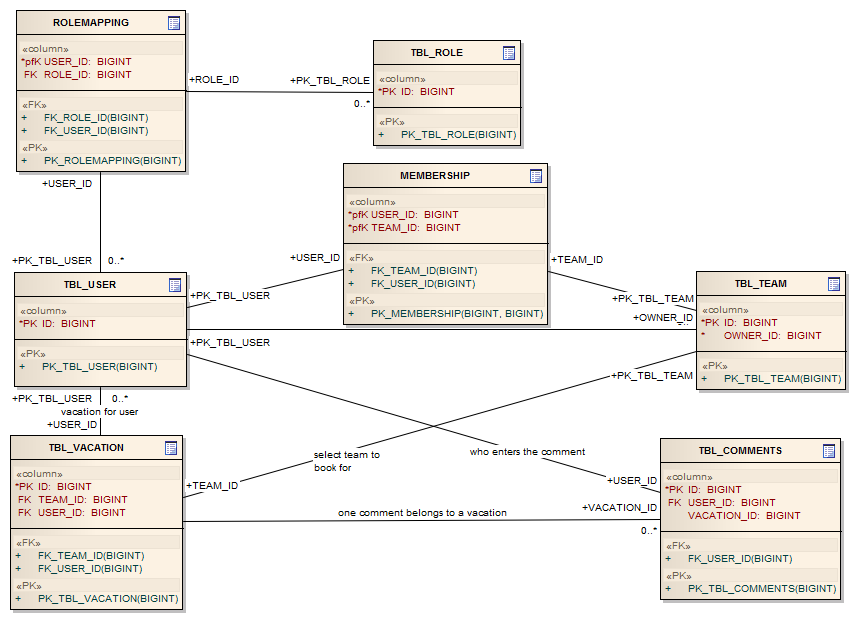
\includegraphics[width=19cm]{images/erm}
        	\caption{Entity Relationship Model}
\end{figure}
\end{landscape}
\subsection{Beschreibung}
Das Entity Relationship Model zeigt alle Tabellen, wie sie auf Ebene der Datenbank geplant sind. Many-to-Many Beziehungen sind in aufgel\"oster Form dargestellt.

\subsubsection{User und Rollen}
Weil Benutzer verschiedene Rollen besitzen und Rollen umgekehrt verschiedenen Benutzern zugeteilt werden k\"onnen, ist die Beziehung TBL\_USER-TBL\_ROLE mittels einer Join-Tabelle ROLEMAPPING aufgel\"ost. Ich habe auf die Implementierung einer Rollenhierarchie verzichtet, trotzdem m\"usste man an deren Implementierung bei einer Business-Anwendung denken. 

\subsubsection{Teammitgliedschaft, Membership}
Die Zuteilung von Membern zu Teams muss ebenfalls \"uber eine Many-to-Many Assoziation realisiert werden. Im Diagramm ist diese durch die Tabelle MEMBERSHIP ersichtlich. 

\subsubsection{Teamzugeh\"origkeit}
Im von mir modelierten einfacheren Fall, bei dem ein Team nur einem Verantwortlichen zugeteilt wird, wird die Beziehung zwischen TBL\_TEAM und TBL\_USER mittels einer One-To-Many Relation hergestellt. Nebst der Einfachheit hat dies den Nachteil, dass Ferien nur vom Administrator (Team-Owner) bewilligt werden k\"onnen, er kann also keine Stellvertreter daf\"ur nominieren. 

\subsubsection{Ferien}
Ferien werden als Eintr\"age in der Tabelle TBL\_VACATION definiert. Die Beziehung zu TBL\_USER ist insofern logisch, da sie immer einem Teilnehmer zugeordnet werden. Die Relation zu TBL\_TEAM definiert, f\"ur welche Gruppe ich meine Ferien beantrage respektive von welchem Verantwortlichen die Ferien bewilligt werden k\"onnen.